\chapter{Background}
This chapter explores the background knowledge that is associated with every other networking concept explored in this document. The next chapters will build upon the foundation that is established here and will use the understanding of the terminology and concepts to address some issues that are also identified here.


\section{Networking principles in games}
Whenever a message is sent over a computer network, there are many different protocols that are used at different stages of the message sending process. Most data that is sent over the internet, is sent over a protocol stack known as TCP/IP, which includes some useful functionality such as the resending of packets if one does not arrive and the reconstruction of a message on the receiving client's end that makes sure the message arrives just as it was sent. While this process works great for content such as websites, the whole process adds a lot of time on top of the data transmission time of each packet. For data that needs to arrive at it's destination as quickly as possible, a more ``bare-bones'' protocol is available; UDP. This is a very simple idea of sending the information packet to it's destination and once it is sent, there is nothing else that the sender needs to do. The problem with sending a UDP packet, is that there is no guarantee when, or if, it will arrive at it's destination. There are many different factors that can cause a given data packet to time-out on it's way to the destination or arrive after taking a sub-optimal route there. The following section explains some potential problems that have to be considered when sending information over any computer network.


\subsection{Communitaction Issues}
In the dissertation \mycite{macedonia1995network}, the author has identified and grouped the most prevalent issues that occur in internet communications. In real time applications such as online games, these issues can be very impactful on the experience of the players.

\subsubsection{Bandwidth}
As \citeauthor{macedonia1995network} explains, ``the available network bandwidth, determines the size and richness of a Virtual Environment''. This is in relation to creating a networked virtual environment, however it also applies to any networking operation. The bandwidth of a network is the limit of how much data can travel through it. The bandwidth required grows exponentially as the size of a peer to peer network expands therefore if large simulations are being run on LAN, the bandwidth could become a limiting factor in that scenario.

\subsubsection{Latency}
The paper \mycite{bettner20011500}, documents the architecture and implementation of networking approaches in the RTS (Real Time Strategy) games ``Age of Empires'' 1 and 2. The authors talk about an experiment that has been performed with the game netcode where players were interviewed on whether they felt that their game inputs felt responsive at different latencies between the players. They have found that when playing with a latency of 250ms or less, the latency was not noticeable at all. Latencies between 250ms and 500ms were ``very playable''. Anything more than 500ms would start becoming noticeable. They have also found that when playing with a noticeable latency, the players have naturally developed a ``mental expectation of the lag'' between the inputs and an action happening. After developing this ``game pace'', they would enjoy playing the game at a consistent, slower response rather than altering between low and high latency.

What can be seen in this example, is that while making the latency between inputs and actions, does make the game more responsive and fun, noticeable jitter when receiving messages can also impact the player's experience in significant ways.


\subsubsection{Reliability}
When a packet is sent out into the network, there is no guarantee that it will be delivered. To fix this principle, the TCP protocol has been created that builds upon UDP. The article \mycite{lincroft1999internet} documents the issues that the development team encountered when developing the netcode for the 1997 game ``X-Wing vs. TIE fighter''. The author has experimented with TCP connections in game data transmission and found that ``TCP refuses to deliver any of the other packets in the stream while it waits for the next "in order" packet. This is why we would see latencies in the 5-second range.'' and ``if a packet is having a tough time getting to its destination, TCP will actually stop re-sending it! The theory is that if packets are being dropped that it's due to congestion.''. The features that have been implemented into TCP to make it reliable, end up negatively effecting real-time application data traffic and due to the volume of data to be transmitted, should not be used for time sensitive data.


\subsection{Inconsistent ping between players}
There are many different possible reasons for the lag to the server to vary widely from player to player. Firstly, it is possible that there are not enough servers throughout the world or that they are not spread out evenly enough across all regions. Players who live in geographically more remote locations, are likely to experience higher ping to servers compared to those that live in more densely populated cities due to where the servers are likely to be located. Secondly, there is no way of guaranteeing if the clients are going to be using a wired or a wireless connection to connect to the server. Wireless connections can be much slower and are more likely to introduce other potential problems such as packet loss.

Varying ping between players could lead to a problem of a poor experience for a client with a high ping to the server, as they will receive the updates from the server later than every other player and therefore be at a disadvantage if the game requires real time reactions. Unfortunately under some implementations, this also results in a poor experience for the other players too, who despite having reasonable ping to the server, can find the game rules to be unfair towards them. For example in a competitive FPS (First Person Shooter) game that ``favours the shooter'', a low ping player can be shot from behind cover by a laggy player who fired a shot before the cover was reached on their version of the game state, which is delayed compared to others' versions.


\subsubsection{Possible solutions to the variable ping problem}
Netcode developers of the most popular games, have tried many different solutions to fix or at least mitigate the issue of widely differing ping to the game server between players. One example of a solution here could be ``region locking''. This is the idea that only players with equally low ping, can connect to the same game instance on a server. This could be done by providing game servers spread out across as many geographical regions as possible and only allow players to connect to their local one. This presents two main issues however. Firstly, this prevents players in different geographical regions from playing together and therefore separates the community. Also, the issue of players in remote areas playing together and having a suboptimal experience due to the server lag, has not been addressed. The developers of Battlefield 1 have implemented an interesting solution to this problem which will be discussed further on in Section \ref{sec:bf1_ping}.


\newpage
\section{Networking Model Options}
There are several different ideas that exist as a solution to the problem of synchronising multiple game clients over a network. The three that are most relevant to this document are the centralised (and distributed) server model, the client hosted model and the peer to peer model. Game netcode developers have to choose one, or multiple, of these implementations when designing their networking logic. Each model has both positive and negative attributes and in the following sections, they will be discussed.


\subsection{The Centralised Server Model}
Most AAA online multiplayer games that are played today, make use of the ``centralised server model'' for synchronising the simulation state between several clients participating in the same simulation. This means that in an example of a First Person Shooter (FPS), if one player presses the ``jump'' key, their character will jump on their screen. This input information would then also be sent over to the game server. The server would then send the information that this player has jumped, to all other clients. There is a potential problem here however. Given that the ping between the server and client A is \(\alpha\) and between the server and client B is \(\beta\), the time between client A pressing an input and client B being notified of this input can not be less than $\alpha+\beta$ and due to the limitations of physics $\alpha>0$ and $\beta>0$. This means that at any given time the lag experienced between clients A and B will be more than $\alpha+\beta$ when aspects such as server tick-rate or network congestion are factored in too.

\begin{figure}[!h]
  \begin{tabular}{ c p{0.94\textwidth} }
    \faCheckCircle & Hardware is likely to be powerful enough to handle the stress of many simulations running simultaneously. \\
    \faCheckCircle & High bandwidth connection is likely to be used. Minimises the chance of high latency and network issues. \\
    \faCheckCircle & Ping to the server is likely to be similar for all players making the game more fair.  \\
    \faCheckCircle & No client can see the address of any other client. \\
    \faCheckCircle & The developer has a lot of control over what is allowed within the game. This allows for anti-cheating systems that are hard to bypass. \\
    \  & \  \\
    \faTimesCircle & Expensive to rent out, or buy and maintain, server space. Letting players rent out servers makes the game more expensive for them. \\
    \faTimesCircle & Many servers have to be spread out evenly throughout the world to allow for low latency connections.  \\
    \faTimesCircle & People living in remote locations may not have low latency access to official servers.
  \end{tabular}
  \caption{The attributes of the central server model}
  \label{fig:cs_attributes}
\end{figure}



\subsection{Client Hosted Model}
The client hosted model is an example of implementing a networking infrastructure without the need for expensive server rental. One of the main advantages of this solution is the idea that one codebase can be written to work as a client hosted model and this codebase can then be adjusted slightly to work on a central server as well if there ever is a need for this in the future. The basic idea behind this implementation method, is that one of the clients, would act as a server for all other participants alongside also being one of the participants. One of the biggest problems with an implementation like this, is that the player that is hosting the game will have a connection to the server with the ping and latency of 0 which will give them an objective advantage in scenarios where quick reaction times are needed. Another potential concern with an implementation like this, is that the player hosting the game, is likely to have consumer grade, lower-end hardware and network connection. It is also possible that a WiFi connection would be used increasing the chance of packet loss and high latency further. There is also a security concern with any networking application that, in order to function, has to know the IP address of every player that is connected. This information can be easily used to determine the country or even the city that the player is connecting from. It would also be possible to find out information about their hardware or network connection through how frequently a packet arrives from this player. A difficulty can also arise if the host player loses connection to the other players as either the game has to finish or a ``host migration'' would have to take place which is a difficult problem.

\begin{figure}[!h]
  \begin{tabular}{ c p{0.94\textwidth} }
    \faCheckCircle & There are no additional costs to the publisher/developer when releasing the game. \\
    \faCheckCircle & Players in remote locations can play together with low latency. \\
    \faCheckCircle & The codebase is relatively easily transferable to a central server model if the need arises. \\
    \  & \  \\
    \faTimesCircle & The host player has negligible ping to the server. This could be a large advantage.  \\
    \faTimesCircle & The host player is likely to use a consumer grade connection increasing the risk of packet loss and high latency \\
    \faTimesCircle & The host player could be using WiFi to host the game which could significantly increase the chance of packet loss. \\
    \faTimesCircle & The host's hardware may not be powerful enough to calculate each simulation step within an acceptable tick rate. \\
    \faTimesCircle & If the host player is disconnected mid-game, a host migration will have to take place pausing the game for a few seconds or causing the game to finish unexpectedly. \\
    \faTimesCircle & The host player can see the IP address of each other player that they are playing with. \\
    \faTimesCircle & Cheating could be easy if the host player sends malicious packets to the clients pretending to be the game server.

  \end{tabular}
  \caption{The attributes of the client hosted model}
  \label{fig:ch_attributes}
\end{figure}



\subsection{Peer to Peer Model}
The idea behind the peer to peer model, is that if two clients can communicate directly, the latency in the connection between them, could be reduced if where wasn't a server that all messages have to go through. The theory here is that the latency between players can be as low as theoretically possible which should result in more responsive gameplay. The use of the peer to peer model is often reserved for applications where only a few clients need to communicate with one another and therefore is a common choice for fighting games and RTS (Real Time Strategy) Games.

For the peer to peer model to work, each client (peer), needs to know the IP address of every other client. This presents a potential security risk as any player in the same instance of the simulation, can use the IP address to determine what country, and sometimes city, each client is connecting from. Another potential problem arises with how the information about each client is distributed to each client. One potential idea of how this could be done, is to have a central server that manages sessions and matchmaking. Clients that are looking for a session with an open spot, would send a join request message to this known server address. This server would match players up based on factors such as player skill. Once enough players have requested to join to start the simulation, the server would broadcast the IP and Port of each client to each other client. From that point, each client has all the information that it needs to start the simulation execution.

If the goal of using the peer to peer model is to avoid the need for server rental or maintenance, this process could also be done with one of the players hosting the game and having the other players know the address of this hosting client. With this setup, the scenario presented above, would work too.

Since each player is communicating with every other client, there is no central ``real state'' of the simulation and due to latency in connections, the simulation from each player's perspective could differ slightly. This also means that each client is responsible for maintaining their own state of the simulation. Another consequence of contacting other clients directly, is that in a randomly selected sample of players in a game that is available worldwide, the latency between each player is likely to vary largely. This can often result in having a slower response when interacting with one player than another who could have a lower latency to you. This could make the game feel unresponsive at times seemingly out of nowhere during gameplay.

The paper \mycite{Carter2009} provides an example of a game called ``Panzer Battalion'', where ``each peer computes its own game version, no player is having disadvantages because of high network lags''. This is an example of a game that uses the peer to peer model to allow for players to play together. The authors also explain that removing a central point of failure, an implementation like this has led to ``contradicting game states'' which could potentially ruin the game experience.


\begin{figure}[!h]
  \begin{tabular}{ c p{0.94\textwidth} }
    \faCheckCircle & There are no additional costs to the publisher/developer when releasing the game. \\
    \faCheckCircle & Players in remote locations can play together with low latency. \\
    \faCheckCircle & There is no concept of host advantage, like what is present with the client hosted model. \\
    \faCheckCircle & Host migrations are not a large problem since everyone has the full simulation state. \\
    \  & \  \\
    \faMinusCircle & Each client communicates directly with other clients making their connection as efficient as possible in theory. \\
    \faMinusCircle & Even though a central ``authority'' is not needed, one of the peers often has to act as a session host to handle invitations and handshakes. \\
    \faMinusCircle & Every client runs it's own simulation and is tasked with keeping it updated with everyone else's. \\
    \  & \  \\
    \faTimesCircle & The lack of a central authority (such as a game server) makes cheat prevention difficult. \\
    \faTimesCircle & Each player in an instance, can see the IP address of every other player they are playing with. \\
    \faTimesCircle & Interacting with two different peers with different latencies, will feel inconsistant for the player.  \\
    \faTimesCircle & Very high bandwidth usage compared to other models. \\
    \faTimesCircle & The amount of update messages that need to be sent, increases as the number of players grows. \\
    \faTimesCircle & A player with a poor internet connection or underpowered hardware, will make the game feel less responsive to other players. \\
   \end{tabular}
  \caption{The attributes of the peer to peer model}
    \label{fig:p2p_attributes}
\end{figure}



\chapter{Related work}
The purpose of this chapter, is to investigate how networking is implemented in popular modern AAA games. To further the research in this topic, an analysis of the development process of using the networking tools available in the Unity game engine will be done.

\section{Networking implementations in games}\label{sec:net_in_games}

\subsection{Variable ping system in Battlefield 1} \label{sec:bf1_ping}
An interesting approach to the issue of variable ping in a game has been implemented by DICE in the game Battlefield 1. Given 2 players; player A with a low ping to the server and player B with a ping of <150ms to the server.

When player B fires at a moving player A, player B's client will perform the check concluding that player A has been hit and this information is sent to the server. The server will then perform it's own checks and if the server agrees that this hit is possible, then it sends the hit confirmation to player B and damage information to player A. This approach is called Clientside-Server Authoritative as while the hit registration is calculated on clientside, the server must still confirm that this is valid.

Considering another scenario, suppose that player A still has a low ping to the server but player B, now has the ping of >150ms. An icon will appear on player B's UI showing an ``aim-lead'' indicator. Now when the shot is fired in the same scenario, the hit will not register anymore as the hit registration has switched from Clientside-Server Authoritative to Fully-Server Authoritative, meaning that the check is performed only once the shot information is received by the server.

Whilst this implementation makes the game feel less responsive for players with high ping, it provides a lot more fairness for everyone else and allows for players with different pings play in a more fair way.


\subsection{Networking in Apex Legends}
Apex Legends is a ``Battle Royale'' game by Respawn Entertainment. Due to the genre of this game, the implementation of networking has been implemented in an interesting way. The premise of the game consists of a starting amount of 60 players, all competing to be the last one alive at the end. An interesting aspect of this, is that while at the start of a match, the server might have to work quite hard to effectively synchronise the simulation for 60 different clients, as more and more players die off and less are left, less information needs to be sent to each of the clients, freeing up some server performance.

Since transferring all the information about 60 different players would most likely exceed the average MTU and therefore slow down the sending process, with each update, the server sends 1 smaller packet per each player to each player. This means that when 60 players are in the game, 60 packets are sent to 60 different clients from the same server. This is shown in the Netcode analysis in \mycite{bns2019apex}.

An interesting outcome of this, is quite noticeable network lag that slowly goes away, as less and less players remain in the game. It is also likely due to this, that Respawn felt the need to implement a ``Client Authoritative'' aiming model. Meaning that the server will favour what the client sees over it's own view of the simulation (i.e. If the client claims that a shot has hit an enemy, the server is likely to agree). The choice for this implementation could have been made to fix two potential issues; reducing the load on the server by reducing the need to perform extensive checks for each shot (this could be significant if a lot of players are playing), making the game feel more responsive on slower client hardware that may need more time to process up to 60 packets that arrive from the server at each update tick.

\subsection{Destiny 2's uniquely complicated netcode}
In 2015, a Bungie developer gave an interesting talk at GDC (Game Developer's Conference): \mycite{truman2015destiny2}. The game Destiny 2, has decided to use the peer to peer model to create an ``always online'' world that players could join and leave freely. This resulted in a netcode that was referred to by \citeauthor{truman2015destiny2} as having a  ``uniquely complicated network topology''. In a previous Bungie game with multiplayer networking, Halo Reach,  a mixture of a peer to peer model and client hosted model has been used in multiplayer matches. Each player would send information such as weapon fire or movement to all other players but there would also be a physics server running on one of the clients in the simulation. The matches were designed to be relatively short and players where incentivised to remain in the game until the end of each match. This meant that if the player running the physics server were to leave, the gameplay flow would have to be interrupted for all other players as the host migration system allocated a new player to run this server. Fortunately, due to the nature of the game, this happened rarely as players were incentivised to remain till the end of the match. In Destiny 2 however, there are many zones (referred to in the talk as ``bubbles'') that a player would often join and leave as they move around the environment. This made host migrations much more common and would happen roughly ``every 160 seconds''. This has prompted Bungie to abandon the client hosted physics server aspect of Destiny 2's netcode and move towards renting cloud server space to host the physics engine. In ``private bubbles'', however, it became inefficient to communicate with a central server for game physics calls so the old system was used there. In summary, Destiny 2 uses peer to peer in order to send packets directly to other players to make the gameplay feel more responsive than sending messages to the server and then a client but has fixed some issues that the game could have if it was fully peer to peer by implementing elements that use client hosted and central server models too.

\begin{figure}[!h]
  \centering
  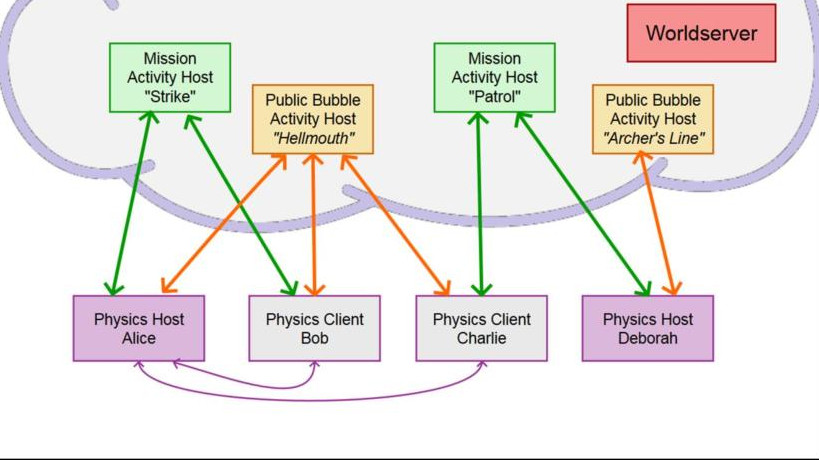
\includegraphics[width=0.5\textwidth]{Destiny2_networking}
  \caption{Example of how netcode is designed in Destiny 2. Image from the GDC talk: \mycite{truman2015destiny2}}
  \label{fig:destiny2netcode}
\end{figure}

\subsection{Issues with the peer to peer system}
The largest issues plaguing the games implemented with the peer to peer system all can be traced back to inconsistencies of state between the peers. This is inevitable when a delay is present in communication between parties. The paper \mycite{Carter2009} discusses some possible solutions that aim to mitigate or eliminate the idea of desynchronised game state. ``In general, during network communication, it can sometimes be assumed that the connection is reliable however we can not assume that messages will arrive in the same order as they are sent''.

The first idea that is suggested is called ``dead reckoning''. The paper \mycite{smed2002review} discusses this topic in detail. This is the idea of estimating what value is likely to be received from the server in the next packet by evaluating the previous values. In an example of an entity moving through a virtual environment at a constant speed in a constant direction and given that the position of this entity is being broadcasted from another entity, the game client can predict that if the previous packets have updated the position of this entity by the same amount every time, it can calculate the next value that will be received before the packet even arrives. This information can be used to interpolate the position of this entity between the packet that has just arrived and what position it is expected to be in after the next packet arrives, thus giving the client a more smooth simulation. This also makes the smoothness of the simulation less reliant on network quality, though with low quality networking, the issue of ``rubber banding''\footnote{Rubber Banding is when a client sees an object in a simulation in a certain location but after a update of where this object should be arrives from an authority (server), this position is instantly updated to this new, correct position. From the client's point of view, this looks like the entity has teleported to the new location.} can become prevalent.

Another idea suggested is called ``local lag'' which involves the idea of putting incoming packets into a queue before they are used in the game. Using this method, if packets arrive out of order, they can be put in-order in the local buffer. In some game implementations, two actions performed in different order could result in a different outcome (for example rotating a character and moving them forwards). A potential downside that can arise from using this method however, involves the fact that additional delay is incorporated to the process of sending information. This makes use of a system like this in games that require timely reactions potentially degrading for the players' experience. Local lag can be implemented in conjunction with dead reckoning for potentially better results however.

Finally, an option called ``time warp'' can be utilised for synchronising game state. This technique is often used and well known in the field of Parallel and distributed Discrete Event Simulation (PDES). The paper \mycite{Jefferson1985} explains this topic in detail and ``Time Warm Mechanism'' is well explained. This mechanism listens and applies updates received from other peers when they arrive, however, periodic ``snapshots'' of the entire game state are saved. If an inconsistency is observed (for example if a straggler message is received from another peer), a ``rollback'' is applied to reset the simulation to a previous state, before the inconsistency was observed. The system would also have to assume that any messages sent before the rollback was performed, were done so under inaccurate assumptions. If this is the case, the peer can send a ``null-message'' which would inform the other peers of the inconsistency and lead them to performing their own ``rollbacks''. This system can often cause ``network floods'' of ``null-messages''.

The system of ``local lag'' assumes that inconsistencies will always occur whereas ``time warp'' can often be considered to be the ``optimistic approach'' because it allows each client to calculate it's simulation state assuming no inconsistencies. Both implementations have uses in different scenarios.

\section{Other networking development tools}
This section houses the research done that is not related to analysing game netcode. Here, other development tools and platforms that are available to developers are explored. The implementation and usage of tools in the Unity engine will also be explored here and will assist in the design of the GNAT library.

\subsection{Google's Stadia and future networking options}
At the Game Developers Conference in March 2019, Google has announced a new Game Streaming platform. The talk outlined the plans that would allow developers to develop games for their Linux based platform that would run the game code on Google servers. Users of this service, would be able to play games by sending their inputs to the google servers. All game logic processing would then take place on the Google servers and the audio and video would be returned to the player. This service could potentially allow players to play games on devices with very little processing power, with settings that would normally require much more power.

A potential unexpected advantage of this system, could allow for networking possibilities that would be difficult to make work with current technologies. If a multiplayer game was developed for this system, it could allow for large scale virtual worlds with many players in the same instance as only one simulation would have to be processed for all the players. Each player's perspective would then be sent to them, this wouldn't be much different from how this system would function in a single player scenario.

The largest potential issue with a system like this could be the latency between the player sending an input to the server and then seeing this input reflected in the output. If this latency can be made negligible through high speed internet connections and high processing power servers, it is possible that a system like this could potentially become a success. Also, if this latency can be minimised, this system could prove to be a model that provides the best networking performance for large scale multiplayer experiences.


\subsection{Networking options in Unity}
A game engine has been described as a core of controlling games by providing the main framework and common functions in the paper \mycite{xie2012research}. Unity is just one example of many different game engines that are available to a developer, which all aim for the same unified goal but try to achieve it in different ways. Unity is a popular choice for projects ranging from small indie titles to large AAA productions and it is known for being relatively easy to use and prototype with. To investigate the options that are available in the market for online game development, I have explored the tools available in the Unity engine. The following sections detail my experience with using the tools.

I have implemented a simple 2D game which allows the player to fire a projectile, jump and move their character left and right. The goal with this project was to go through the process of transforming a simple, single player game to a simple multiplayer game through the use of Unity's official networking library.

\subsubsection{UNET}
The method of networking that I have decided to investigate was Unity's own UNET library. UNET uses the client hosted model that requires one client to act as a game server allowing others to connect to it. The joining clients need to know the IP address of the host in order to connect to them and the host can either join the game themselves or act purely as a server. The figures \ref{fig:unet_ui}, \ref{fig:main} and \ref{fig:in_game}, show screenshots of the default UI that is provided by the library as well as my game showing the main menu, client and server perspectives respectively. The tile-based pixel art used in the game has been found on the Unity Asset Store under the name ``Sunny Land Forest'' and has been designed by Ansimuz.

Initially, the implementation of networking features proved to be very simple. A networking manager had to be added to the main scene and the networked scene had to be chosen. Spawn points, and the order that they should be used in, was easy to configure and the UI that allowed the user to connect and play was a simple addition too. Once two different player characters were spawned in, there were some changes that had to be made to the movement scripts that involved specifying different behaviour whether the given character ``belongs'' to this player, or the other player. Checking if the character belonged to the player was as simple as comparing one boolean. This change can be seen in the change of colour of the character to blue if it is not the player controlled character in figure \ref{fig:in_game}.

When testing this version of the game, I have found that the movement felt just as smooth inside the multiplayer game session as it did in the single player game. When both the host and the client are playing on localhost (this should in theory provide the lowest latency possible for communications), player 1's movement, would be roughly translated to player 2's perspective correctly, however instead of the movement appearing as smooth as it does for the local player's movement, the enemy character seems to teleport around with every frame appearing in a different location in a radius around where they ``should'' be at that time. This could be due to the UNET implementation of dead reckoning that does not predict the upcoming positions very well. This teleportation problem occurs for both the host and the client. Another issue appears when a fast-moving projectile is fired. For the host, all projectiles fly just as they should, in a straight line and colliding with a collider. On the client's screen however, it appears as if the tick-rate of the server cannot keep up with the speed of this projectile. Often there are only 1 or 2 frames when the projectile sprite can be seen flashing on the screen in different positions before not being shown again. This appears to happen for both player's projectiles on the client's game. There is another issue with this implementation of my game on top of this; the desynchronisation of the two players happens very often. After player 2 stops moving, on player 1's screen, player 2's character will continue moving as if a force was being applied in a certain direction on the character collider. This very often results in the two simulations showing completely different states to each other making it hard to know where the other player really is.

All these issues could be fixed by implementing techniques designed for minimising de-sync in peer to peer games and/or sending and reading custom messages between the clients that are designed to work with the game logic, however the default implementation of the official library that is designed to synchronise prefab positions and colliders, appear to work too slowly to be truly useful for quick moving objects, even in the most optimal conditions.

\begin{figure}[p]
  \centering
  \subfloat[Main Menu UI]{
    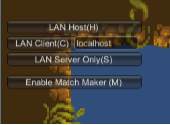
\includegraphics[width=0.3\linewidth]{UNET/Main_Menu_UI}
  }
  \qquad
  \subfloat[Host UI]{
    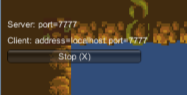
\includegraphics[width=0.3\textwidth]{UNET/Host_UI}
  }
  \qquad
  \subfloat[Client UI]{
    
\includegraphics[width=0.3\linewidth]{UNET/Client_UI}
  }

  \caption{UNET default UI}
  \label{fig:unet_ui}
\end{figure}

\begin{figure}[p]
  \centering
  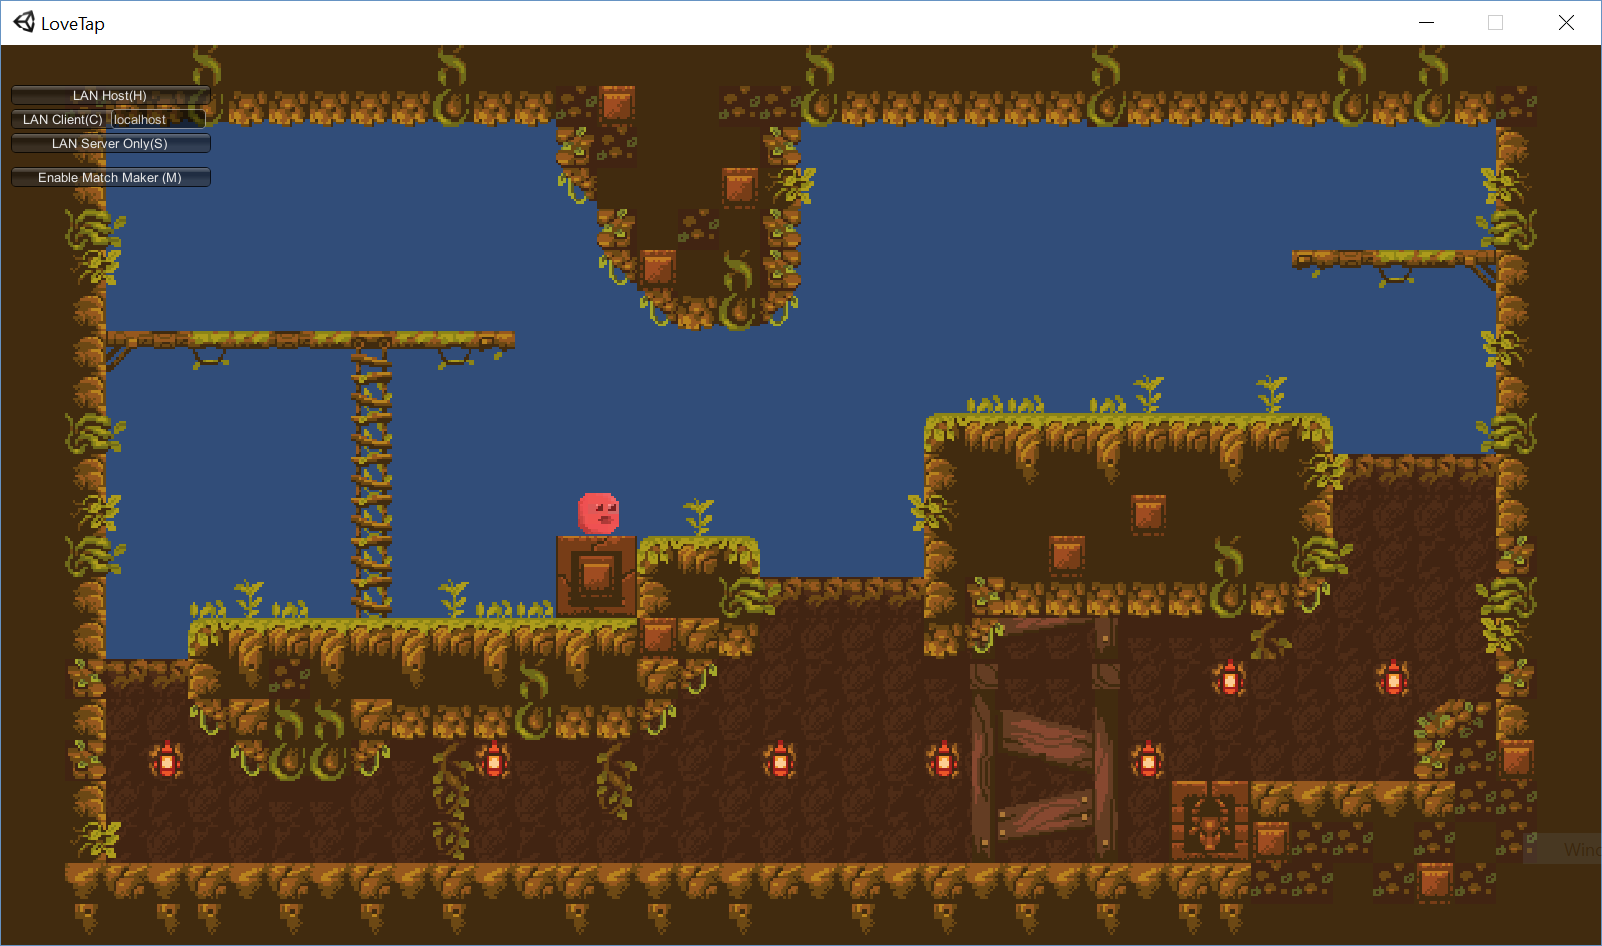
\includegraphics[width=\textwidth]{UNET/Main_Menu}
  \caption{Main Menu}
  \label{fig:main}
\end{figure}


\begin{figure}[p]
  \centering

  \subfloat[Host game screen]{
    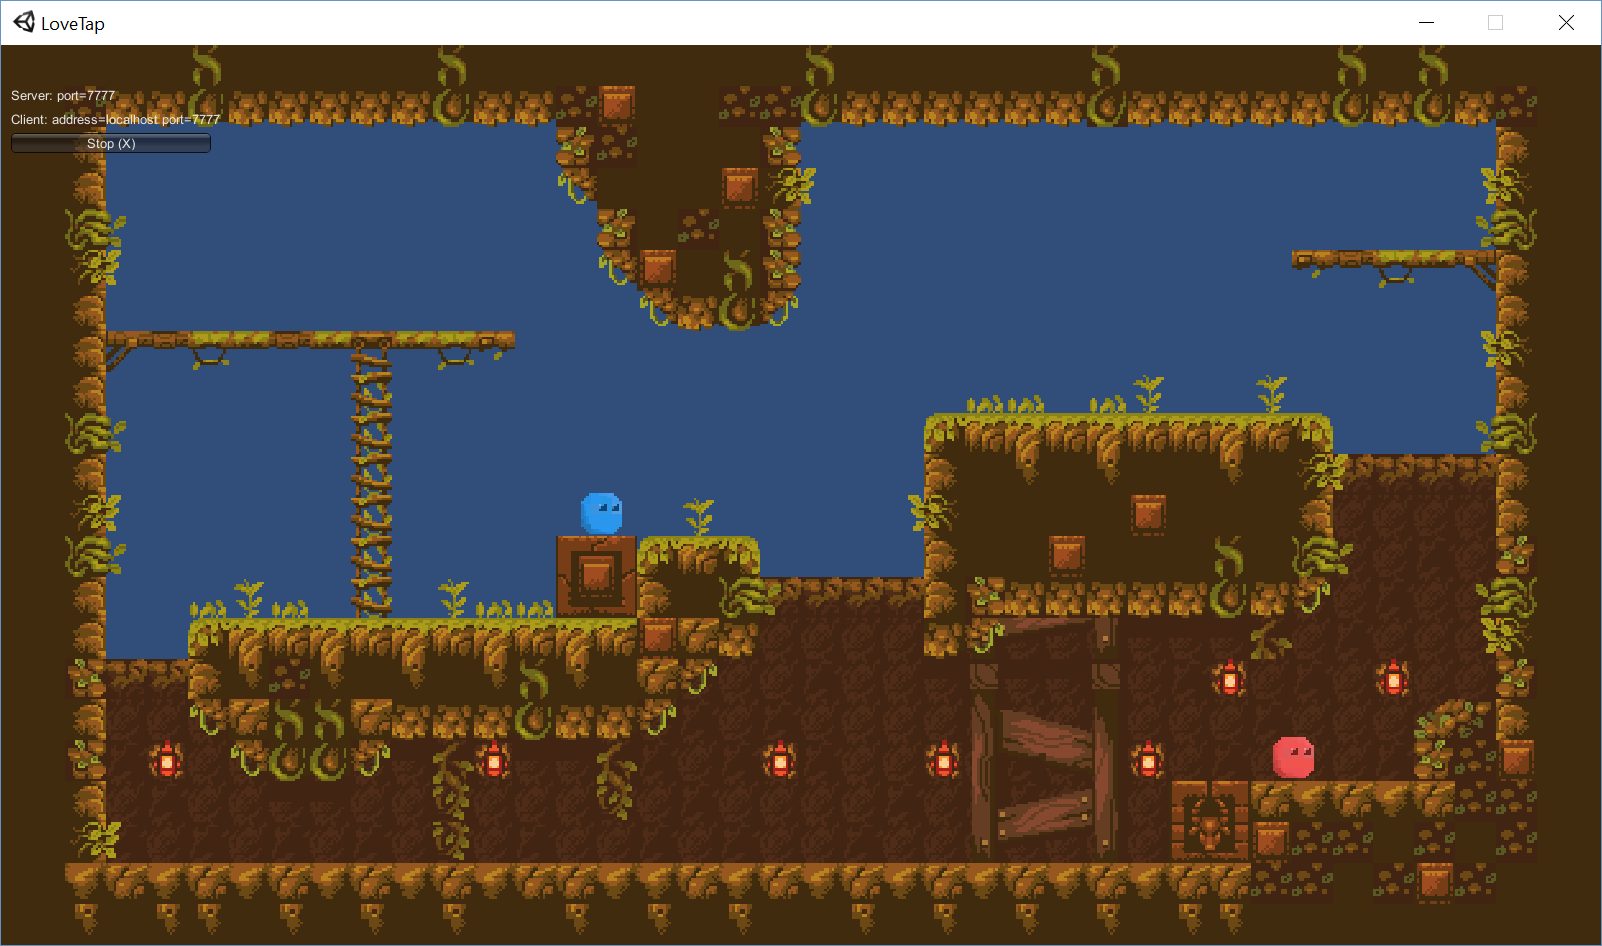
\includegraphics[width=0.45\textwidth]{UNET/Host}
  }
  \qquad
  \subfloat[Client game screen]{
    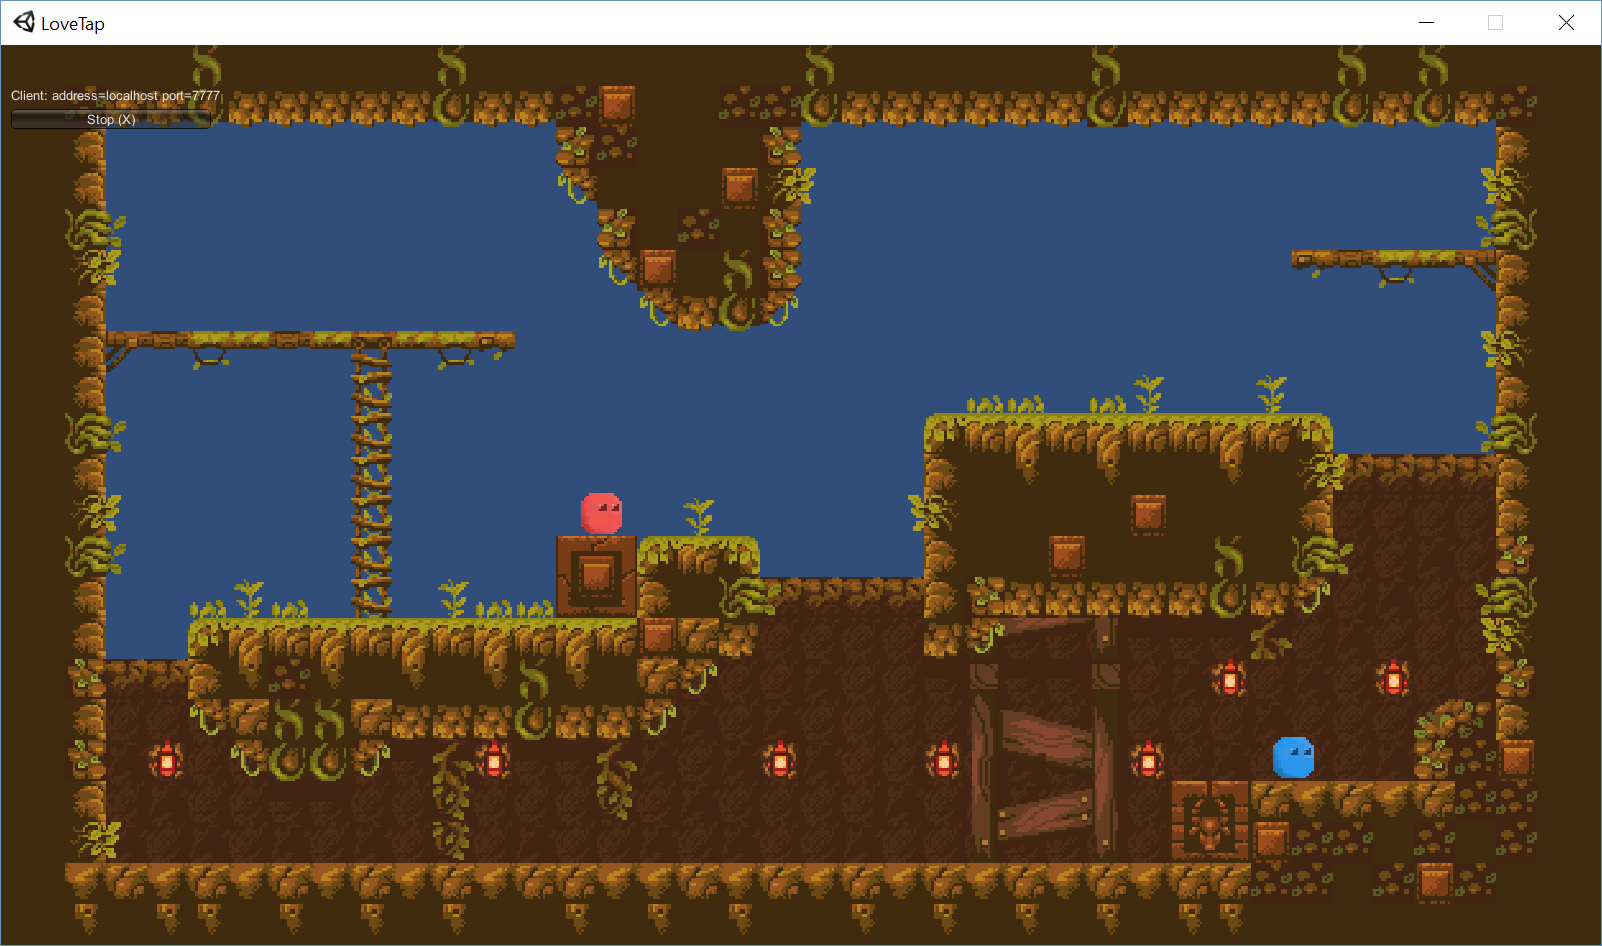
\includegraphics[width=0.45\linewidth]{UNET/Client}
  }

  \caption{Main game loop after connection is established}
  \label{fig:in_game}
\end{figure}

\newpage

\section{Related work summary} \label{sec:related_work_sum}
Most modern high-budget game releases include a competitive multiplayer mode that allow players to challenge their friends or compete with strangers over the internet. The advances in networking architecture allow for seamless multiplayer worlds such as those found in Destiny 2 and the heavily optimised experiences to make the game experience ``feel'' responsive and fair with systems like those implemented in Battlefield 1 are often taken for granted. In fact, the only time an average consumer is likely to think about how netcode is implemented or the systems that come together to make the game feel fluid, is when a networking system is implemented poorly or a system fails in a given scenario. If the system is implemented well, it is not even noticed or thought about.

This chapter has outlined some potential issues that can be encountered when designing netcode for unusual situations and how some netcode architects have tackled these issues. I have then done further research into how an existing network library works so that some insight from it's design can be used in the design of GNAT.
From using UNAT, I have found that through trying to make the library user friendly, the developers have made it hard to customise exactly what information should be synchronised. It was also difficult to use the library to send and receive custom messages, which could've been useful to address some of the experienced issues. In summary, UNET has succeeded in making itself easy to integrate into a project and get simple synchronisation working, however it was hard to customise what was synchronised. When designing the GNAT library, both the strengths and weaknesses of the UNAT library should be considered.
